\documentclass{beamer}
%%%%%% UNOFFICIAL ICL BEAMER TEMPLATE V.0.1 %%%%%%

\usepackage[english]{babel}
\usepackage{amsmath,amssymb}
\usepackage{multirow}
\usepackage{tikz}
\usetikzlibrary{arrows.meta,positioning,fit,backgrounds,calc}

%%%%%% THE FOLLOWING FILE CONTAINS THE STYLE DEFINITIONS %%%%%%
\input{header.tex}
%%%%%%

%%%%%% TITLE, AUTHOR, DATE DEFINITIONS %%%%%%
\title{Decision Theory II \\ {\large Reflective Oracles, Open-Source Games, and Commitment Races}}
\author{Daniel C}
\date{}
%%%%%%

\begin{document}

\frame{\titlepage}

\frame{\frametitle{Where we are: agents that model each other}
	\begin{block}{Two foundational obstacles to mutual modelling}
		{\tiny
		\begin{itemize}
			\item Deck I ended at \textbf{fair computational worlds}: agent and environment are both programs that may inspect, simulate, or predict each other. Embedded agents must model other agents -- including agents like themselves.
			\item This raises two questions, and this deck takes both:
			\begin{itemize}\scriptsize
				\item[(1)] \textbf{Can a Bayesian agent even represent other agents like itself?} Self-modelling failures of AIXI, the \emph{grain of truth} problem, and \emph{reflective oracles}.
				\item[(2)] \textbf{When agents can read each other's code, how do they cooperate without conflict?} Open-source game theory, \emph{commitment races}, and \emph{safe Pareto improvements}.
			\end{itemize}
			\item Punchline preview: reflective oracles solve mutual modelling \emph{semantically} (a shared oracle); open-source games solve it \emph{syntactically} (read the code). Both then face the strategic problem of \emph{commitment}.
		\end{itemize}
		}
	\end{block}
}

%==================================================================
\section{Self-modelling failures \& AIXI}
%==================================================================
% Diagrams in this section are recreated in TikZ after C. Wyeth, Embedded Agency;
% the cybernetic / embedded-agent figures are after the LessWrong Embedded Agency sequence.

\frame{\frametitle{The cybernetic model and large agents}
	\begin{columns}[T]
	\begin{column}{0.56\textwidth}
	\begin{block}{Learn a model, then plan with it}
		{\tiny
		\begin{itemize}
			\item Cybernetic model: an agent \emph{learns a model} of its environment and \emph{plans} with it to achieve a goal.
			\item Two implicit assumptions:
			\begin{itemize}\scriptsize
				\item[(1)] the agent is \textbf{``larger than''} the environment -- its mind can hold a full copy of the world;
				\item[(2)] the agent is \textbf{``outside''} the environment.
			\end{itemize}
			\item Note $1\Rightarrow2$, so model-based RL almost always assumes (2). Can we still reason when the agent is \emph{smaller} than its environment?
		\end{itemize}
		}
	\end{block}
	\end{column}
	\begin{column}{0.44\textwidth}
	\begin{center}
	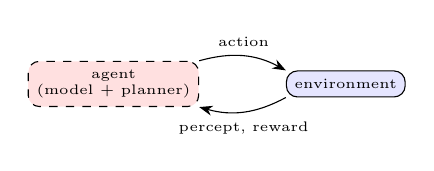
\begin{tikzpicture}[>=Stealth, font=\tiny,
	   b/.style={draw, rounded corners, align=center, inner sep=3pt}]
	  \node[b, fill=red!12, dashed] (ag) {agent\\ (model $+$ planner)};
	  \node[b, fill=blue!10, right=11mm of ag] (env) {environment};
	  \draw[->] (ag.north east) to[bend left=22] node[above,font=\tiny]{action} (env.north west);
	  \draw[->] (env.south west) to[bend left=22] node[below,font=\tiny]{percept, reward} (ag.south east);
	\end{tikzpicture}\\[1mm]
	{\tiny\itshape clean boundary: the agent sits \emph{outside} the world}
	\end{center}
	\end{column}
	\end{columns}
	{\tiny \hfill (Section follows C.~Wyeth, \textit{Embedded Agency}; diagrams recreated, after the LessWrong Embedded Agency sequence.)}
}

\frame{\frametitle{The actual situation: embedded agency}
	\begin{columns}[T]
	\begin{column}{0.54\textwidth}
	\begin{block}{The agent is a part of the world}
		{\tiny
		\begin{itemize}
			\item An agent is \emph{just a special part of} the environment.
			\item It may be \textbf{modified, destroyed, or copied} (by itself or others) between interaction steps.
			\item Other \textbf{equally powerful agents} may exist, \emph{mutually reasoning about each other}.
			\item Safety relevance of getting this right: reward hacking, the shutdown problem, user identification.
			\item Can we reason about an agent \emph{smaller} than, and contained in, its environment?
		\end{itemize}
		}
	\end{block}
	\end{column}
	\begin{column}{0.46\textwidth}
	\begin{center}
	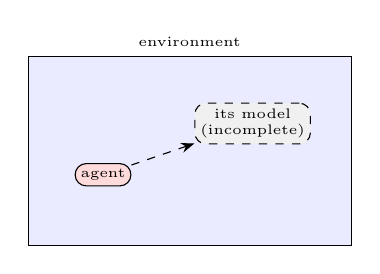
\begin{tikzpicture}[>=Stealth, font=\tiny]
	  \node[draw, fill=blue!8, minimum width=4.1cm, minimum height=2.4cm, label={[font=\tiny]above:environment}] (env) {};
	  \node[draw, fill=red!14, rounded corners, inner sep=2pt, font=\tiny] (ag) at ([shift={(-1.1cm,-0.3cm)}]env.center) {agent};
	  \node[draw, dashed, fill=gray!12, rounded corners, inner sep=2pt, font=\tiny, align=center] (mod) at ([shift={(0.8cm,0.35cm)}]env.center) {its model\\ (incomplete)};
	  \draw[->, dashed] (ag) -- (mod);
	\end{tikzpicture}\\[1mm]
	{\tiny\itshape it cannot fit the whole world (including itself) inside}
	\end{center}
	\end{column}
	\end{columns}
}

\frame{\frametitle{History-based reinforcement learning}
	\begin{columns}[T]
	\begin{column}{0.50\textwidth}
	\begin{block}{The general framework}
		{\tiny
		\begin{itemize}
			\item Under the cybernetic assumption, a very general class of tasks is modelled as \textbf{history-based RL}.
			\item The agent emits actions $a_n$ and receives percepts $e_n=(o_n,r_n)$: observations $o_n$ and rewards $r_n$.
			\item The \emph{interaction history} is the interleaved sequence $a_1 o_1 r_1\, a_2 o_2 r_2\cdots$
		\end{itemize}
		}
	\end{block}
	\end{column}
	\begin{column}{0.50\textwidth}
	\begin{center}
	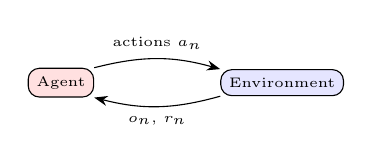
\begin{tikzpicture}[>=Stealth, font=\tiny,
	   b/.style={draw, rounded corners, align=center, inner sep=3pt}]
	  \node[b, fill=red!12] (ag) {Agent};
	  \node[b, fill=blue!10, right=16mm of ag] (env) {Environment};
	  \draw[->] (ag.north east) to[bend left=15] node[above,font=\tiny]{actions $a_n$} (env.north west);
	  \draw[->] (env.south west) to[bend left=15] node[below,font=\tiny]{$o_n$, $r_n$} (ag.south east);
	\end{tikzpicture}\\[3mm]
	{\tiny $\cdots\, a_1 o_1 r_1\ \ a_2 o_2 r_2\ \ a_3 o_3 r_3\, \cdots$}\\[1mm]
	\begin{tikzpicture}[>=Stealth]\draw[->] (0,0)--(2.6,0) node[right,font=\tiny]{time};\end{tikzpicture}
	\end{center}
	\end{column}
	\end{columns}
}

\frame{\frametitle{AIXI}
	\begin{block}{The optimal history-based agent for computable environments [Hut00]}
		{\tiny
		\begin{itemize}
			\item AIXI \textbf{plans optimally against a Bayesian mixture of all programs}: a Solomonoff prior over environment-programs $q$, weighted by simplicity $2^{-\ell(q)}$.
			\item The simplest formulation fits on one line (fixed horizon $m$, iterative value function), writing $e_i=o_i r_i$:
			$$a_k \;:=\; \arg\max_{a_k}\sum_{o_k r_k}\cdots\max_{a_m}\sum_{o_m r_m}\big[r_k+\dots+r_m\big]\!\!\sum_{q:\,U(q,\,a_{1:m})=e_{1:m}}\!\! 2^{-\ell(q)}.$$
			\item Read right-to-left: weight every environment-program $q$ consistent with the chosen actions by $2^{-\ell(q)}$, average the reward, then \emph{expectimax} over actions and percepts. The gold standard of an idealised \emph{dualistic} agent -- but is it \emph{embedded}-ready?
		\end{itemize}
		}
	\end{block}
}

\frame{\frametitle{Joint history prediction: the idea}
	\begin{columns}[T]
	\begin{column}{0.54\textwidth}
	\begin{block}{Predict the whole tape, actions included}
		{\tiny
		\begin{itemize}
			\item Go \emph{beyond} the cybernetic framework by \textbf{jointly predicting the entire history} -- actions and percepts alike.
			\item Formalisation: $a_1 e_1 a_2 e_2\cdots = h \sim \rho$ for a distribution $\rho$ over histories.
			\item The cybernetic assumption is the \emph{special case} $\rho=\mu^{\pi}$: the history factorises into an environment $\mu$ (percepts given actions) and a policy $\pi$ (actions given history).
		\end{itemize}
		}
	\end{block}
	\end{column}
	\begin{column}{0.46\textwidth}
	\begin{center}
	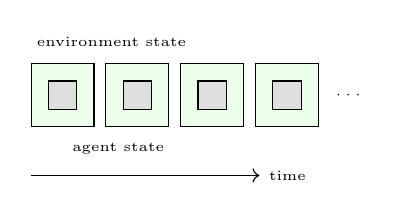
\begin{tikzpicture}[font=\tiny]
	  \foreach \i in {0,1,2,3} {
	    \draw[fill=green!8] (\i*0.95,0) rectangle (\i*0.95+0.8,0.8);
	    \draw[fill=gray!25] (\i*0.95+0.22,0.22) rectangle (\i*0.95+0.58,0.58);
	  }
	  \node[font=\tiny] at (4.05,0.4) {$\cdots$};
	  \node[font=\tiny, anchor=west] at (-0.05,1.08) {environment state};
	  \node[font=\tiny, anchor=west] at (0.4,-0.28) {agent state};
	  \draw[->] (0,-0.62)--(2.9,-0.62) node[right]{time};
	\end{tikzpicture}
	\end{center}
	\end{column}
	\end{columns}
}

\frame{\frametitle{Joint history prediction: Solomonoff's mixture}
	\begin{block}{From pure prediction to a joint belief}
		{\tiny
		\begin{itemize}
			\item For pure prediction, Ray Solomonoff's universal distribution is a Bayesian mixture over all probabilistic programs:
			$$M(x) \;=\!\! \sum_{p:\,U(p)=x*}\!\! 2^{-\ell(p)}\qquad(\text{programs whose output starts with } x).$$
			\item Marcus Hutter extended this to decision problems. The joint AIXI belief is built from $M$ as a product of one-step conditionals:
			$$\xi^{U}(e_{1:t}\,\|\,a_{1:t}) \;=\; \prod_{i=1}^{t} M\big(e_i \mid h_{<i}\,a_i\big).$$
			\item \emph{Why not just use this to predict the joint distribution -- actions and all?}
		\end{itemize}
		}
	\end{block}
}

\frame{\frametitle{Joint history prediction: why it breaks for RL}
	\begin{block}{Joint prediction does not transfer cleanly}
		{\tiny
		\begin{itemize}
			\item Joint prediction does \textbf{not} immediately transfer to RL; learning may \textbf{not converge} even when the cybernetic assumption holds.
			\item One can choose \textbf{uncomputable odd bits} that destroy Solomonoff prediction on the \emph{computable} even bits, e.g.
			$$\mathtt{11}\ \ \mathtt{00}\ \ \mathtt{00}\ \ \mathtt{11}\ \ \mathtt{11}\ \ \mathtt{11}\ \ \mathtt{11}\ \cdots\qquad(\text{odd bits uncomputable, even bits computable}).$$
			\item The same trick: certain \textbf{uncomputable actions} can break Solomonoff \emph{percept} prediction.
			\item Surprisingly, \textbf{normalising $M$} patches this particular problem.
		\end{itemize}
		}
	\end{block}
}

\frame{\frametitle{Semimeasure loss}
	\begin{columns}[T]
	\begin{column}{0.52\textwidth}
	\begin{block}{The missing probability mass}
		{\tiny
		\begin{itemize}
			\item $M$ is only a \textbf{semimeasure}: probability can \emph{leak} (as if the sequence may ``stop''),
			$$\nu(x)\;\ge\;\sum_{a\in\Sigma}\nu(xa)\quad(\text{a measure has equality}).$$
			\item There are several ways to \emph{complete} / \emph{normalise} a semimeasure: reallocate the leftover gap among the continuations.
			\item The gap reallocated this way is the \textbf{semimeasure loss}.
		\end{itemize}
		}
	\end{block}
	\end{column}
	\begin{column}{0.48\textwidth}
	\begin{center}
	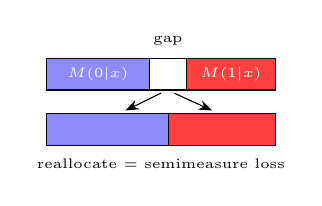
\begin{tikzpicture}[>=Stealth, font=\tiny]
	  \fill[blue!45] (0,0.7) rectangle (1.3,1.1); \draw (0,0.7) rectangle (1.3,1.1); \node[white,font=\tiny] at (0.65,0.9) {$M(0|x)$};
	  \draw[fill=white] (1.3,0.7) rectangle (1.78,1.1);
	  \fill[red!75] (1.78,0.7) rectangle (2.9,1.1); \draw (1.78,0.7) rectangle (2.9,1.1); \node[white,font=\tiny] at (2.34,0.9) {$M(1|x)$};
	  \node[font=\tiny] at (1.54,1.32) {gap};
	  \fill[blue!45] (0,0) rectangle (1.55,0.4); \draw (0,0) rectangle (1.55,0.4);
	  \fill[red!75] (1.55,0) rectangle (2.9,0.4); \draw (1.55,0) rectangle (2.9,0.4);
	  \draw[->] (1.45,0.66)--(1.0,0.44); \draw[->] (1.62,0.66)--(2.1,0.44);
	  \node[font=\tiny] at (1.45,-0.24) {reallocate $=$ semimeasure loss};
	\end{tikzpicture}
	\end{center}
	\end{column}
	\end{columns}
}

\frame{\frametitle{Prediction of selected bits}
	\begin{block}{The semimeasure loss can be large infinitely often}
		{\tiny
		\begin{itemize}
			\item The semimeasure loss can be made \emph{large infinitely often} [Lattimore--Hutter--Gavane].
			\item \textbf{Theorem 7 (adversarial non-convergence of $\xi^{U}$)} [Wyeth--Hutter]: there exists $e=a\in\mathbb{B}^{\infty}$ such that
			$$\xi^{U}(e_{1:t}\,\|\,a_{1:t}) \;=\; \xi^{U}(a_{1:t}\,\|\,a_{1:t}) \;\longrightarrow\; 0 \quad\text{as } t\to\infty.$$
			\item Reading: there are histories where, even though the reward has \emph{always} matched the (binary) value of the action, AIXI \textbf{infinitely often doubts} this will continue.
			\item \emph{Caution:} we do not know whether these (action) histories are \emph{on-policy} for AIXI. And Theorem 7 \textbf{fails when $M$ is normalised.}
		\end{itemize}
		}
	\end{block}
}

\frame{\frametitle{AIXI is much ``larger'' than its environment}
	\begin{columns}[T]
	\begin{column}{0.57\textwidth}
	\begin{block}{The agent is not in its own hypothesis class}
		{\tiny
		\begin{itemize}
			\item AIXI believes the environment is \textbf{lower semicomputable} ($\Sigma^0_1$).
			\item But AIXI's own \emph{policy} is \textbf{not} lower semicomputable -- it sits \emph{higher} in the arithmetical hierarchy:
			$$\cdots\,\Delta^0_n \subset \Sigma^0_n,\Pi^0_n \subset \Delta^0_{n+1} \subset \Sigma^0_{n+1},\Pi^0_{n+1}\,\cdots$$
			\item Hence \textbf{``AIXI does not believe the universe contains AIXI agents.''}
		\end{itemize}
		}
	\end{block}
	\end{column}
	\begin{column}{0.43\textwidth}
	\begin{center}
	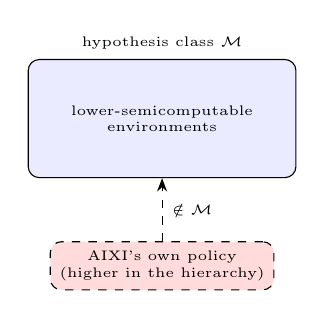
\begin{tikzpicture}[>=Stealth, font=\tiny]
	  \node[draw, rounded corners, fill=blue!8, minimum width=3.4cm, minimum height=1.5cm, align=center, label={[font=\tiny]above:hypothesis class $\mathcal{M}$}] (M) {lower-semicomputable\\ environments};
	  \node[draw, dashed, rounded corners, fill=red!14, font=\tiny, align=center, below=8mm of M] (pi) {AIXI's own policy\\ (higher in the hierarchy)};
	  \draw[->, dashed] (pi) -- node[right, font=\tiny]{$\notin\mathcal{M}$} (M);
	\end{tikzpicture}
	\end{center}
	\end{column}
	\end{columns}
}

%==================================================================
\section{The grain of truth problem \& reflective oracles}
%==================================================================

\frame{\frametitle{Modeling multi-player games}
	\begin{columns}[T]
	\begin{column}{0.54\textwidth}
	\begin{block}{Mutual modelling needs same-size agents}
		{\tiny
		\begin{itemize}
			\item Agents which are modelling each other must be of the \textbf{``same size''}.
			\item Therefore AIXI \textbf{cannot learn} that the environment contains other AIXI instances.
			\item Note: multi-player games do \emph{not} necessarily involve other embedded-agency problems (``being inside the environment'') -- this obstacle is specifically about \emph{mutual modelling}.
		\end{itemize}
		}
	\end{block}
	\end{column}
	\begin{column}{0.46\textwidth}
	\begin{center}
	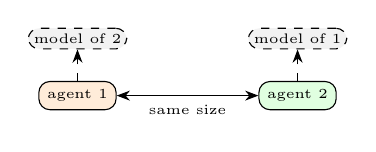
\begin{tikzpicture}[>=Stealth, font=\tiny,
	   b/.style={draw, rounded corners, align=center, inner sep=3pt},
	   m/.style={draw, dashed, rounded corners, fill=gray!10, inner sep=2pt, font=\tiny}]
	  \node[b, fill=orange!15] (A) {agent 1};
	  \node[b, fill=green!12, right=18mm of A] (B) {agent 2};
	  \node[m, above=4mm of A] (mA) {model of 2};
	  \node[m, above=4mm of B] (mB) {model of 1};
	  \draw[->,dashed] (A)--(mA); \draw[->,dashed] (B)--(mB);
	  \draw[<->] (A)--(B) node[midway,below,font=\tiny]{same size};
	\end{tikzpicture}\\[1mm]
	{\tiny\itshape each must fit a model of the other -- as powerful as itself}
	\end{center}
	\end{column}
	\end{columns}
}

\frame{\frametitle{The grain of truth problem}
	\begin{block}{Correctly-specified subjective models}
		{\tiny
		\begin{itemize}
			\item In a multiplayer game we want each Bayesian player to have a \emph{correctly-specified} model of its subjective environment: never \textbf{``infinitely surprised''} by an event that has positive probability under the true history distribution.
			\item Given a class of games $\mathcal{G}$, a class of strategies $\mathcal{P}$, and subjective beliefs $\xi_i$ for player $i$, the \textbf{grain of truth property} requires:
			\begin{itemize}\scriptsize
				\item[--] each optimal policy $\pi^{*}_{\xi_i}\in\mathcal{P}$ (the best response stays in the class), and
				\item[--] each belief $\xi_i \gg \sigma^{\pi}$ for all $\sigma\in\mathcal{G},\ \pi\in\mathcal{P}^{n}$,
			\end{itemize}
			where $\gg$ denotes \textbf{absolute continuity} (the truth is absolutely continuous w.r.t.\ the belief; by Blackwell--Dubins, posteriors then \emph{merge}).
		\end{itemize}
		}
	\end{block}
}

\frame{\frametitle{Solution with reflective oracles (I): the construction}
	\begin{columns}[T]
	\begin{column}{0.60\textwidth}
	\begin{block}{Precise access to others, without hanging}
		{\tiny
		\begin{itemize}
			\item This appears to \textbf{fail for AIXI players}. Naively, build games/policies by
			$$\lambda_T(x_t\mid x_{<t}) = \mathbb{P}[\,T(x_{<t})=x_t\,],$$
			but \textbf{policies hang} when they call each other (infinite regress).
			\item Instead, give each machine $T$ a \textbf{reflective oracle} $O$ giving \emph{arbitrarily precise access} to the RHS for all other machines $T'$ that also use $O$:
			$$\lambda^{O}_T(x_t\mid x_{<t}) = \mathbb{P}[\,T^{O}(x_{<t})=x_t\,].$$
			\item $O$ \emph{reflects} the true probability and may \textbf{randomise} exactly at the query threshold, so nothing hangs and no liar paradox arises (such $O$ exists -- Fallenstein--Taylor--Christiano). These augmented machines build a \textbf{reflective AIXI} with the grain of truth property.
		\end{itemize}
		}
	\end{block}
	\end{column}
	\begin{column}{0.40\textwidth}
	\begin{center}
	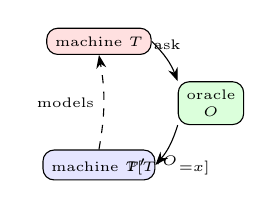
\begin{tikzpicture}[>=Stealth, font=\tiny,
	   b/.style={draw, rounded corners, align=center, inner sep=3pt}]
	  \node[b, fill=red!12] (T) {machine $T$};
	  \node[b, fill=blue!10, below=12mm of T] (Tp) {machine $T'$};
	  \node[b, fill=green!14, right=10mm of $(T)!0.5!(Tp)$] (O) {oracle\\ $O$};
	  \draw[->] (T.east) to[bend left=12] node[above,font=\tiny]{ask} (O.north west);
	  \draw[->] (O.south west) to[bend left=12] node[below,font=\tiny]{$\mathbb{P}[T'^{O}{=}x]$} (Tp.east);
	  \draw[->, dashed] (Tp.north) to[bend right=10] node[left,font=\tiny]{models} (T.south);
	\end{tikzpicture}\\[1mm]
	{\tiny\itshape randomise at the threshold $\Rightarrow$ no hang}
	\end{center}
	\end{column}
	\end{columns}
}

\frame{\frametitle{Solution with reflective oracles (II): results}
	\begin{block}{What reflective oracles buy}
		{\tiny
		\begin{itemize}
			\item \textbf{Game-theoretic results:}
			\begin{itemize}\scriptsize
				\item[--] in the ``dualistic'' multiplayer setup: convergence to \textbf{Nash equilibrium} in stage games, and generally convergence to optimality for \textbf{Thompson sampling} [Leike--Taylor--Fallenstein; Wyeth et al.];
				\item[--] if we allow \emph{correlations} between policies (joint prediction): provable \textbf{``acausal'' coordination} in the Prisoner's Dilemma [Meulemans et al.].
			\end{itemize}
			\item The \textbf{semimeasure loss is eliminated} and prediction of selected bits \emph{succeeds}.
		\end{itemize}
		}
	\end{block}
}

\frame{\frametitle{Solution with reflective oracles (III): self-modelling}
	\begin{block}{Using the self-model -- and its limits}
		{\tiny
		\begin{itemize}
			\item An agent can \textbf{exploit its self-model to avoid planning}; in principle this lets it \emph{reason about self-modifications}.
			\item However, it is \textbf{difficult to prove optimality} (or any other interesting property) of this model. With the oracle-based joint belief $a_1 e_1 a_2 e_2\cdots\sim\xi^{O}$:
			$$\pi_S(h_{<t}) \in \arg\max_{a_t}\ \xi^{O}\!\Big(\textstyle\sum_{i=t}^{\infty}\gamma_i r_i \,\Big|\, h_{<t}\,a_t\Big).$$
			\item \textbf{Bridge to the rest of the deck:} reflective oracles solve mutual modelling \emph{semantically} (a shared oracle); open-source game theory does it \emph{syntactically} -- the agents read each other's source code.
		\end{itemize}
		}
	\end{block}
}

%==================================================================
\section{Open-source game theory}
%==================================================================

\frame{\frametitle{A 60-second refresher on game theory}
	\begin{columns}[T]
	\begin{column}{0.60\textwidth}
	\begin{block}{Nash, and the Prisoner's Dilemma}
		{\tiny
		\begin{itemize}
			\item A (normal-form) game: players, action sets, and payoffs $u_i(a_1,\dots,a_n)$ depending on the \emph{joint} action.
			\item \textbf{Nash equilibrium:} a profile where no player gains by deviating \emph{alone}.
			\item \textbf{Prisoner's Dilemma:} $(C,C)$ is better for both than $(D,D)$, yet $D$ \emph{dominates} $C$ for each player. The unique Nash is $(D,D)$: rational players defect, and both end up worse.
			\item \textbf{Root cause:} your payoff depends on the \emph{joint} action, but you must choose \emph{without knowing or affecting} the other's choice. You cannot \emph{condition} on what they do.
		\end{itemize}
		}
	\end{block}
	\end{column}
	\begin{column}{0.40\textwidth}
	\begin{center}
	{\tiny
	\renewcommand{\arraystretch}{1.25}
	\begin{tabular}{cc|c|c|}
	 & & \multicolumn{2}{c}{\textbf{Player 2}}\\
	 & & $C$ & $D$\\
	\cline{3-4}
	\multirow{2}{*}{\rotatebox{90}{\textbf{P1}}}
	 & $C$ & $3,3$ & $0,5$\\
	\cline{3-4}
	 & $D$ & $5,0$ & $1,1$\\
	\cline{3-4}
	\end{tabular}
	}
	\vskip2mm
	{\tiny\itshape $(D,D)$ is the only Nash, though $(C,C)$ beats it for both.}
	\end{center}
	\end{column}
	\end{columns}
}

\frame{\frametitle{L\"obian cooperation: FairBot}
	\begin{block}{When players can read each other's code}
		{\tiny
		\begin{itemize}
			\item \textbf{Open-source (program) game} (Tennenholtz): each player submits a \emph{program} that takes the opponent's \emph{source code} as input and outputs an action. Now you \emph{can} condition on the opponent.
			\item \textbf{FairBot:} ``cooperate iff I can \emph{prove} my opponent cooperates with me.''
			\item \textbf{FairBot vs.\ FairBot:} by \textbf{L\"ob's theorem}, each proves mutual cooperation and so cooperates. (Here L\"ob is a \emph{feature}: $\Box(\Box C \to C)\to\Box C$, the self-referential proof search succeeds.) Two mutually suspicious agents cooperate, just by reading each other.
			\item \textbf{Unexploitable:} FairBot cooperates with CooperateBot, but \emph{defects} against DefectBot (it cannot prove a defector cooperates). It is never the sucker.
			\item Caveat: proof-based FairBot is \emph{brittle} -- it depends on syntactic provability, can fail to prove cooperation with a differently-written but behaviourally-cooperative bot, and proof search may not terminate.
		\end{itemize}
		}
	\end{block}
}

\frame{\frametitle{Robust cooperation by simulation: $\varepsilon$-grounded bots}
	\begin{block}{Replacing proofs with simulation (Oesterheld)}
		{\tiny
		\begin{itemize}
			\item \textbf{$\varepsilon$-grounded FairBot:} with small probability $\varepsilon$, cooperate \emph{unconditionally} (``ground out''); with probability $1-\varepsilon$, \emph{run the opponent's program} on your own code and \emph{copy} its action.
			\item \textbf{Why it terminates:} each level of mutual simulation grounds out with probability $\varepsilon$, so the recursion halts with probability $1$ -- no infinite regress (contrast the naive ``run each other'' that hangs).
			\item Two $\varepsilon$-grounded FairBots (almost always) cooperate, and this is a \textbf{Nash equilibrium} of the program game. It is \textbf{robust}: programs that \emph{behave} the same are treated the same (unlike syntactic proof-based bots).
			\item (The $\varepsilon$-grounded $\pi$Bot and its generalisations, arXiv:2412.14570, prove folk theorems for such simulation-based equilibria.)
		\end{itemize}
		}
	\end{block}
}

\frame{\frametitle{What open-source game theory is really doing}
	\begin{block}{Conditional commitment}
		{\tiny
		\begin{itemize}
			\item Two desiderata for a good decision theory here:
			\begin{itemize}\scriptsize
				\item[(1)] \textbf{cooperate with your own copy}, and
				\item[(2)] \textbf{unexploitability} -- an opponent cannot become better off by making you worse off.
			\end{itemize}
			\item Why ordinary game theory fails: payoff depends on the joint action, but you are uncertain about the opponent's action and they about yours -- a chicken-and-egg of \emph{mutual uncertainty}.
			\item \textbf{Open-source game $=$ conditional commitment:} ``\emph{I commit to $X$ conditional on you committing to $Y$.}''
			\begin{itemize}\scriptsize
				\item[--] the \textbf{conditional} part keeps you \emph{unexploitable} (you cooperate only if they do);
				\item[--] the \textbf{commitment} part makes your cooperation \emph{legible}, so you can satisfy the conditions of the opponent's conditional commitment.
			\end{itemize}
			\item FairBot is exactly this: ``I commit to $C$ conditional on a proof that you commit to $C$.''
		\end{itemize}
		}
	\end{block}
}

%==================================================================
\section{Commitment races}
%==================================================================

\frame{\frametitle{The commitment races problem}
	\begin{block}{Why consequentialists race to commit (Kokotajlo)}
		{\tiny
		\begin{itemize}
			\item A consequentialist (acts purely on expected consequences) is both a \textbf{bully and a coward}: it threatens when threats work, and \emph{caves} to credible threats. So \textbf{whoever commits first controls the one who commits later}.
			\item This creates a \textbf{race}: it pays to commit \emph{before} you have thought or learned -- to ``move first''. For agents that read or simulate each other, even \emph{thinking longer} leaks exploitable information about what you will do.
			\item Two catastrophe modes:
			\begin{itemize}\scriptsize
				\item[--] \textbf{Incompatible commitments lock in:} both players throw out the steering wheel in a game of Chicken $\Rightarrow$ a crash neither wanted (e.g.\ grim-trigger protocols keyed to incompatible bargaining solutions).
				\item[--] \textbf{Wasteful racing:} everyone commits before learning -- a coordination failure like an arms race.
			\end{itemize}
		\end{itemize}
		}
	\end{block}
}

\frame{\frametitle{Moving first in logical time; and s-risks}
	\begin{block}{Why this is a safety priority}
		{\tiny
		\begin{itemize}
			\item ``First'' is not clock time but \textbf{logical time}: who, in the structure of mutual prediction, effectively decides \emph{before} the other. An agent that is \emph{predicted} to have committed \emph{is} committed -- even simultaneously in clock time.
			\item \textbf{Connection to s-risks (risks of astronomical suffering).} The most dangerous commitments are \emph{threats}: ``do $X$ or I make things very bad for you.'' Commitment races can lock superintelligences into \emph{carrying out} catastrophic threats (or executing them to build credibility), i.e.\ suffering on an astronomical scale.
			\item So a decision theory that avoids commitment races -- letting agents reach good outcomes \emph{without} a destructive scramble to pre-commit -- is a genuine safety goal, not a curiosity.
		\end{itemize}
		}
	\end{block}
}

\frame{\frametitle{Influencer vs.\ responder}
	\begin{columns}[T]
	\begin{column}{0.60\textwidth}
	\begin{block}{The first-mover's advantage, and the race it triggers}
		{\tiny
		\begin{itemize}
			\item \textbf{Responder:} run the opponent's program, observe its action, then $\arg\max$ your own utility against that action (a plain \emph{best response}).
			\item \textbf{Influencer:} \emph{assume the opponent is a responder} (will best-respond to you); $\arg\max$ your utility over that -- i.e.\ pick the point on the Pareto frontier \textbf{best for you and worst for the opponent}, knowing they will cave.
			\item \textbf{``The best response is not the best response'':} being a naive best-responder is \emph{dominated} by being the influencer. So everyone wants to be the influencer $\Rightarrow$ a race to ``move first in logical time''.
		\end{itemize}
		}
	\end{block}
	\end{column}
	\begin{column}{0.40\textwidth}
	\begin{center}
	\begin{tikzpicture}[>=Stealth, font=\tiny]
	  \draw[->] (0,0)--(3,0) node[right]{$u_{1}$};
	  \draw[->] (0,0)--(0,3) node[above]{$u_{2}$};
	  \draw[blau-upc, thick] (0.3,2.7) to[bend left=18] (2.7,0.3);
	  \node at (1.5,2.6) {\tiny Pareto frontier};
	  \fill[red] (2.45,0.55) circle (1.6pt);
	  \node[right, font=\tiny, text=red!70!black] at (2.0,0.95) {influencer's pick};
	\end{tikzpicture}
	\vskip1mm
	{\tiny\itshape moves first $\Rightarrow$ grabs its favourite corner of the frontier}
	\end{center}
	\end{column}
	\end{columns}
}

\frame{\frametitle{The generalized commitment race: entanglement}
	\begin{block}{Why agents are not incentivised to make Pareto improvements}
		{\tiny
		\begin{itemize}
			\item When you choose your program in an open-source game, you optimise against your \emph{subjective distribution} over the opponent's possible programs -- including \textbf{counterfactual} ones (programs they might have submitted but didn't).
			\item So you cannot simply maximise against the opponent's \emph{actual} program: doing so might make you worse off against \emph{counterfactual} versions. Your incentive is \textbf{entangled} with those counterfactual programs.
			\item Equivalently: whenever a rational agent ``\emph{punishes}'' an opponent (for, say, proposing a Pareto improvement), it is \emph{forgoing utility against the actual program} to gain utility against some \emph{counterfactual} program.
			\item \textbf{Entanglement is the obstacle:} it is exactly what disincentivises accepting a Pareto improvement (accepting might look ``soft'' and cost you against a counterfactual hawk). This is the \emph{generalized} commitment race -- it persists even with full conditional commitment.
		\end{itemize}
		}
	\end{block}
}

%==================================================================
\section{Safe Pareto improvements}
%==================================================================

\frame{\frametitle{Safe Pareto improvements (SPI)}
	\begin{block}{Improving on a default that risks conflict}
		{\tiny
		\begin{itemize}
			\item Setup (Oesterheld--Conitzer; DiGiovanni--Clifton--Mac\'e, arXiv:2403.05103): players delegate to \emph{representative} programs. The \emph{default} instruction is ``play the original game as best you can''.
			\item An \textbf{SPI} is a re-instruction (restrict the strategy set, or re-map utilities) that is \textbf{guaranteed to make \emph{every} player weakly better off} -- with \emph{no} probabilistic assumptions about how the representatives play. A Pareto improvement that is \emph{safe} because it improves \emph{regardless} of the opponent.
			\item Example: a game heading for costly conflict (Chicken-style). Agree on a transformation that strips out the mutually destructive outcome; each player does at least as well, whatever happens.
			\item The paper proves a clean guarantee -- the \textbf{Pareto Meet Minimum (PMM)}: each player gets at least their \emph{lowest payoff over efficient (Pareto-optimal) outcomes}, and this bound is \emph{tight} (renegotiation cannot promise more). Next slide: why. Caveat: it needs a strong assumption.
		\end{itemize}
		}
	\end{block}
}

\frame{\frametitle{Why an SPI guarantees a floor: the Pareto Meet Minimum}
	\begin{columns}[T]
	\begin{column}{0.58\textwidth}
	\begin{block}{The shape of the renegotiation set controls exploitation}
		{\tiny
		\begin{itemize}
			\item Each agent's \emph{renegotiation set} is the Pareto-improvements it will accept. On the frontier, ``better for the opponent'' \emph{means} ``worse for me''.
			\item Let $A$ be the frontier point \textbf{best for me} (worst for the opponent). I have every reason to include points \emph{up to} $A$: pushing the opponent below $A$'s level cannot help me -- by definition $A$ already maximises \emph{my} payoff on the frontier.
			\item But including points \emph{beyond} $A$ (where I would accept being worse than at $A$) enables \textbf{exploitation}: the opponent could make herself better off by making me worse off.
			\item So rational renegotiation sets stop at each player's $A$-point. The worst the agreed outcome can be for me is the \emph{opponent's} $A$-point -- my \textbf{lowest efficient payoff}. That guaranteed floor is the \textbf{PMM} (and it is tight).
		\end{itemize}
		}
	\end{block}
	\end{column}
	\begin{column}{0.42\textwidth}
	\begin{center}
	\begin{tikzpicture}[>=Stealth, font=\tiny]
	  \draw[->] (0,0)--(3.2,0) node[right]{$u_{1}$};
	  \draw[->] (0,0)--(0,3.2) node[above]{$u_{2}$};
	  \draw[blau-upc, very thick] (0.6,2.6) to[bend left=18] (2.6,0.6);
	  \fill[red] (2.6,0.6) circle (1.6pt); \node[above right,font=\tiny,text=red!70!black] at (2.45,0.62) {$A$: best for me};
	  \fill[blue] (0.6,2.6) circle (1.6pt); \node[above right,font=\tiny,text=blue!70!black] at (0.6,2.55) {$A'$: best for opp.};
	  \draw[dashed,gray] (0.6,2.6)--(0.6,0);
	  \node[font=\tiny,align=center] at (1.35,0.2) {my floor\\ $u_1(A')$};
	\end{tikzpicture}\\[1mm]
	{\tiny\itshape accept the frontier between $A'$ and $A$, never beyond}
	\end{center}
	\end{column}
	\end{columns}
}

\frame{\frametitle{The assumption SPI relies on -- and the cheating problem}
	\begin{block}{Participation independence}
		{\tiny
		\begin{itemize}
			\item \textbf{Participation independence:} representatives behave the \emph{same} in the SPI-transformed game as in the default game -- their play does not change just because an SPI is in effect. This independence is what lets you \emph{guarantee} the improvement.
			\item But it is unrealistic. \textbf{The cheating problem:} if I know that an SPI will Pareto-improve away any conflict, then conflict is \emph{less costly} for me, so I am incentivised to submit a \emph{more hawkish} default program.
			\item Anticipating my hawkishness, my opponent's incentive to offer the SPI in the first place is undermined. \textbf{The SPI can defeat itself} -- precisely the entanglement effect, reappearing.
		\end{itemize}
		}
	\end{block}
}

\frame{\frametitle{Entanglement-free SPI: the idea}
	\begin{block}{Make the improvement with an entanglement-free program}
		{\tiny
		\begin{itemize}
			\item Diagnosis: \emph{entanglement} (caring about counterfactual opponent programs) is what disincentivises Pareto improvements. So make the improvement using a separate program that is \textbf{entanglement-free} -- the \textbf{renegotiation program}.
			\item \textbf{Sequential structure:} agents \emph{first} exchange renegotiation programs and \emph{update on the actual one}; \emph{then} submit their default programs.
			\item Because you update on the opponent's \emph{actual} renegotiation program, you optimise against \emph{it}, not against counterfactual versions $\Rightarrow$ \emph{no entanglement} $\Rightarrow$ no incentive to punish/reject improvements.
			\item The renegotiation program may \emph{only propose Pareto improvements} (conditional on the opponent's default program). Two consequences:
			\begin{itemize}\scriptsize
				\item[--] it can \emph{never make the opponent worse off} $\Rightarrow$ no influencer-responder exploitation, \emph{even though} it moves first;
				\item[--] it \emph{conditions on the default program} $\Rightarrow$ it can \emph{detect} hawkish ``cheating'' defaults and withhold improvements, restoring unexploitability and \textbf{removing reliance on participation independence}.
			\end{itemize}
			\item You keep your full action space: you can still play the open-source game with your default program; the renegotiation program only \emph{adds} the option to Pareto-improve.
		\end{itemize}
		}
	\end{block}
}

\frame{\frametitle{Entanglement-free SPI: the protocol}
	\begin{columns}[T]
	\begin{column}{0.56\textwidth}
	\begin{block}{A clean formalism}
		{\tiny
		\begin{itemize}
			\item Open-source game: actions $A=A_1\times A_2$, utilities $u_i:A\to\mathbb{R}$, programs $p_i:P_{-i}\to A_i$, joint action $a=\big(p_1(p_2),\,p_2(p_1)\big)$.
			\item \textbf{Renegotiation function} $rn_i:RN_{-i}\times A\to\mathcal{C}(A)$: conditional on the opponent's renegotiation function, it proposes a \emph{set} of Pareto-improvements on the default outcome $a$. A rule $\mathrm{sel}$ picks one point of the agreed intersection.
			\item \textbf{Entanglement-free renegotiation program} $en_i:P_{-i}\to RN_i$ reads the opponent's \emph{default} program, outputs a renegotiation function.
			\item The intersection $I = rn_1(rn_2,a)\cap rn_2(rn_1,a)$ holds the Pareto-improvements \emph{both} agents will make; $\mathrm{sel}(I)$ is the final outcome. (Choosing $\mathrm{sel}$ adds no coordination problem, under mild conditions -- DiGiovanni.)
		\end{itemize}
		}
	\end{block}
	\end{column}
	\begin{column}{0.44\textwidth}
	\begin{center}
	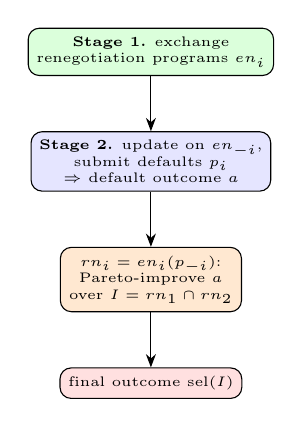
\begin{tikzpicture}[>=Stealth, font=\tiny,
	   b/.style={draw, rounded corners, align=center, inner sep=3pt, minimum width=23mm}]
	  \node[b, fill=green!14] (s1) {\textbf{Stage 1.} exchange\\ renegotiation programs $en_i$};
	  \node[b, fill=blue!10, below=7mm of s1] (s2) {\textbf{Stage 2.} update on $en_{-i}$,\\ submit defaults $p_i$\\ $\Rightarrow$ default outcome $a$};
	  \node[b, fill=orange!18, below=7mm of s2] (s3) {$rn_i=en_i(p_{-i})$:\\ Pareto-improve $a$\\ over $I=rn_1\cap rn_2$};
	  \node[b, fill=red!12, below=7mm of s3] (s4) {final outcome $\mathrm{sel}(I)$};
	  \draw[->] (s1)--(s2); \draw[->] (s2)--(s3); \draw[->] (s3)--(s4);
	\end{tikzpicture}
	\end{center}
	\end{column}
	\end{columns}
}

\frame{\frametitle{Why first-mover is safe here -- and what we trade away}
	\begin{block}{Resolving the race without creating a new one}
		{\tiny
		\begin{itemize}
			\item Usually, a sequential structure creates an influencer-responder race (the first mover grabs the frontier). Here the first move (renegotiation) can \emph{only Pareto-improve}, so it \textbf{cannot exploit} -- no new commitment race is introduced.
			\item Net result: entanglement-free SPI \textbf{solves the cheating problem} and \textbf{drops the participation-independence assumption} (the renegotiation program conditions on the defaults to catch cheating), while the sequential structure \textbf{avoids introducing its own commitment race}.
			\item \textbf{The trade-off -- no tight PMM.} The renegotiation program conditions on the default program, so it can create an \emph{incentive gradient}: ``more cooperative default $\Rightarrow$ I offer more Pareto-improvement; more hawkish $\Rightarrow$ less''. Because it may \emph{withhold} improvement to shape the opponent's default, the agreed set is no longer the full ``up-to-$A$'' set, and the tight \textbf{Pareto Meet Minimum} floor is lost. Weaker (more realistic) assumptions buy a weaker guarantee.
		\end{itemize}
		}
	\end{block}
	{\tiny \hfill (Entanglement-free SPI: Daniel C; selection-function coordination after DiGiovanni.)}
}

\end{document}
